% Document class and packages
\documentclass[letterpaper, 12pt]{article}
\usepackage[utf8]{inputenc}
\usepackage[T1]{fontenc}
\usepackage{geometry}
\usepackage{titlesec}
\usepackage{enumitem}

\usepackage{amsmath, amssymb,lipsum,fancyhdr,graphicx,listings,xcolor,array}

% Page setup
\geometry{margin=1in}
\pagestyle{fancy}
\fancyhf{}
\rhead{\thepage}
\lhead{\textit{Audio \& Image Compression - Assignment 3 - Audio}}  % Escape '&' with '\&'

% Section and list formatting
\titleformat{\section}[block]{\normalfont\Large\bfseries}{\thesection}{1em}{}[]
\setlist[itemize]{left=0pt, label=--, itemsep=4pt}

% Document information
\title{Audio \& Image Compression}
\author{Bashar Beshoti (207370248)
}
\date{\today}

\begin{document}

% First page: Course details and author information
\maketitle

\section*{Course Information}
\begin{itemize}
    \item \textbf{Course Title:} Audio \& Image Compression  % Escape '&' with '\&'
    \item \textbf{Course Code:} 203.3880
    \item \textbf{Assignment :} Final assignment - Audio
    \item \textbf{Due Date : } 04.04.2024

\end{itemize}

\definecolor{dkgreen}{rgb}{0,0.6,0}
\definecolor{gray}{rgb}{0.5,0.5,0.5}
\definecolor{mauve}{rgb}{0.58,0,0.82}

\lstset{frame=tb,
  language=Python,
  aboveskip=3mm,
  belowskip=3mm,
  showstringspaces=false,
  basicstyle={\small\ttfamily},
  numbers=none,
  numberstyle=\tiny\color{gray},
  keywordstyle=\color{blue},
  commentstyle=\color{dkgreen},
  stringstyle=\color{mauve},
  breaklines=true,
  tabsize=3,
  frame=single
}

\newpage

\section{ Dual-Tone Multi-Frequency – DTMF}
\paragraph{Background :}DTMF signals have been used to represent 16 and 50 characters for many years in telephony.
For the purpose of representing these 16 characters are used in two signals at different frequencies. When one frequency is selected from the low range of
The frequencies and it represents the row and the second frequency is chosen from the upper domain and it represents the column. In total there are
Four frequencies in each field and this allows the representation of 16 different characters.
The following table shows the representation of the aforementioned 16 characters:

\begin{table}
    \centering
    \begin{tabular}{|>{\centering\arraybackslash}p{0.1\linewidth}|>{\centering\arraybackslash}p{0.1\linewidth}|>{\centering\arraybackslash}p{0.1\linewidth}|>{\centering\arraybackslash}p{0.1\linewidth}|>{\centering\arraybackslash}p{0.1\linewidth}|} \hline 
         &  Column I - 1209HZ&  Column II - 1336HZ&  Column III - 1477HZ& Column IV - 1209HZ\\ \hline 
         ROW I - 697HZ&  1&  2&  3& A\\ \hline 
         ROW II - 770HZ&  4&  5&  6& B\\ \hline 
         ROW III - 852HZ&  7&  8&  9& C\\ \hline 
         ROW IV - 941HZ&  \#&  0&  *& D\\ \hline
    \end{tabular}
    \caption{DTMF Table}
\end{table}

The first three columns are familiar to us from every phone and the last column is for future use.\\
Now let's say we want to create a DTMF signal that represents the number "5". We will create a sinusoidal signal with a frequency of 770 hz and connect it with a sinusoidal signal at a frequency of 1336 hz (the number 5 is in the second column, second row)
And the result will be the displayed signal:
\begin{figure}[htbp]
    \centering
    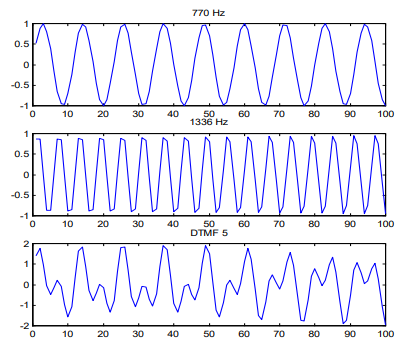
\includegraphics[width=0.5\linewidth]{FINAL_ASSIGNMENT/A_Q_1.png}
    
    
\end{figure}
\subsection{Which of the following spectral images is best suited to represent the number "5"? You have to reason!}
\paragraph{Answer :} \textbf{Diagram 2}. \\
According to the table above, digit "5" create a sinusoidal signal with a frequency of 770 hz
and connect it with a sinusoidal signal at a frequency of 1336 hz (the number 5 is in the second column, second row). since, the diagram shows a high amplitude over 780 hz and 1327 hz which are the closest waves are to 770 hz and 1336 hz. Depending to magnitude level on the digram below, we notice that 780hz and 1327 hz high altitude that is close to the two frequencies of "5" given by the table above.
\begin{figure}[htbp ]
    \centering
    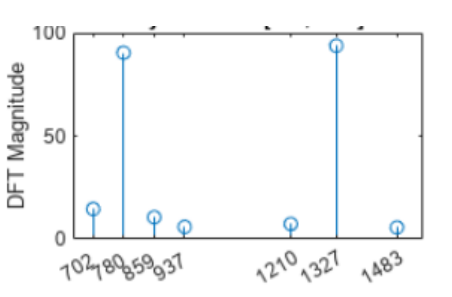
\includegraphics[width=0.5\linewidth]{FINAL_ASSIGNMENT/A_A_1.png}
    \caption{Diagram II}
\end{figure}



\subsection{DTMF signals are chosen so that no frequency is a multiple of another frequency in the table and the distance between each two :}

\textbf{1. Frequencies is not equal to any frequency in the table, It must be explained why in your opinion it was done this way.} Explain!

\paragraph{Answer :} 
\textit{Definition : Harmonic Interference - a harmonic of a wave is a component frequency of the signal that is an integer multiple of the fundamental frequency.\\}

To prevent what is known as Harmonic collision and audio ambiguity. In signal processing,  If one frequency was a multiple of another, it could produce harmonics that might be mistaken for another signal entirely or it may create ambiguity. This could lead to incorrect character detection or interference Mitigation or even audio misinterpretation.


\subsection{When talking on the phone and simultaneously transmitting DTMF signals:} 
\paragraph{1. Can DTMF signals interfere with speech on the phone?\\} 
Despite that DTMF tones are designed to be distinct from the human voice in terms of their frequency. Upon using phone and simultaneously transmitting DTMF signals, it might interfere with speech during a phone call. As upon press a button, the phone generates two tones at specific frequencies. These tones might be heard in the background while you speak especially with no pre-processing and post-processing the audio during call transmission. for example, The higher the volume amplitude of the tones, the more likely they interfere with speech on phone.

\paragraph{2. Can talking on the phone interfere with DTMF signals?\\} 
The phone might also interfere with DTMF signals under certain circumstances. The interference is usually minimal, telephony systems are engineered to prioritize the clarity and integrity of DTMF signals, employing techniques such as signal processing algorithms and noise cancellation to minimize any potential interference from background noise or speech. However, with background noise, distortions, it can potentially interfere with the DTMF signals.

\subsection{DTMF and LPC encoder:} 
\paragraph{1. Will they be transmitted well through a standard LPC encoder?} 
LPC encoding is effective for compressing speech signals, it may not be suitable for transmitting DTMF signals. DTMF signals consist of dual tones representing two sinusoidal signals and have distinct frequency components. LPC encoding, optimized for speech signals, might not accurately preserve the frequency components and temporal characteristics of DTMF signals. Therefore, transmitting DTMF signals through a standard LPC encoder may result in distortion or even loss of the DTMF signal information, making it unreliable for DTMF signal transmission.

\paragraph{2. A correct DTMF decoder must detect a signal that lasted at least mSec40 and reject signals?} 
\begin{enumerate}
    \item Minimum Signal Duration (mSec40): A correct DTMF decoder needs the signal to last at least 40 milliseconds (ms) to reliably identify the two tones. This ensures enough time for accurate frequency analysis.
    \item Maximum Signal Duration (mSec20 for Rejection): Signals shorter than 20 ms are likely not intended DTMF tones. They could be noise bursts, button presses that didn't fully connect, or other transient events. Rejecting these short signals helps prevent misinterpretations.
\end{enumerate}

\paragraph{3. Which costs less than mSec20. What do you think is the reason for this?} 
This requirement is to allow the system to distinguish between separate DTMF signals. If two signals were sent too close together, they might blur into one another, making it difficult for the system to accurately detect the start and end of each signal. Within a minimum interval of 50 milliseconds between signals, the system can ensure that each signal is clearly separated and can be accurately detected and decoded.

\paragraph{4. Between two adjacent signals there must be an interval of at least mSEc50 - what is the reason for this In your opinion ?} A minimum interval of 50 ms between adjacent DTMF signals is required for a few reasons:

Button Release Time: It takes some time to fully release a button after pressing it. A 50 ms gap ensures the previous tone has completely faded before the next one starts, preventing overlap that could lead to decoding errors.
Filtering: DTMF decoders might employ filters to isolate DTMF tones from background noise. These filters, especially those designed for lower sampling rates, need some time to settle between signals for accurate detection. The 50 ms gap allows for the filters to respond effectively, considering typical sampling rates used in telephony (e.g., 8 kHz).


\subsection{Propose a system to detect only DTMF signals (there is no presence of speech) - a clear general scheme must be for such a system (decoding only)}

\paragraph{System Description :} 
\begin{enumerate}
    \item \textbf{Signal Acquisition:} The system first needs to acquire the signal. This could be done through a microphone or directly from a digital source.
    \item \textbf{Pre-processing}: The acquired signal may need some preprocessing. This could include filtering out noise and normalizing the signal.
    \item \textbf{Frequency Detection}: The system then needs to detect the frequencies present in the signal. This could be done using a Fast Fourier Transform (FFT) or other spectral analysis techniques. The goal is to identify the two frequencies that make up the DTMF signal.
    \item \textbf{DTMF Decoding}: Once the two frequencies have been identified, the system can then decode the DTMF signal. This involves mapping the pair of frequencies to the corresponding DTMF character. This could be done using a lookup table or other data structure that stores the frequency pairs and their corresponding characters. 
    \item \textbf{Post-processing}: After the DTMF character has been decoded, the system may perform some post-processing. This could include error checking or other validation to ensure the decoded character is valid.
    \item \textbf{Output}: Finally, the system outputs the decoded DTMF character. This could be displayed on a screen, stored in a file, or used as input to another system.
\end{enumerate}

\paragraph{Scheme :}
\begin{figure}[htbp]
    \centering
    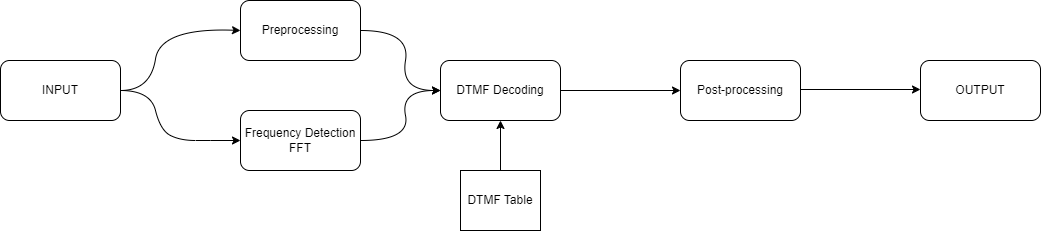
\includegraphics[width=0.85\linewidth]{FINAL_ASSIGNMENT/A_Q_5.png}
    
    
\end{figure}



\subsection{Based on everything we have seen so far - let's say that a decoder system is required that should receive a normal transmission (telephony) or (as described in the previous section) - a transmission with only DTMF signals - try to propose an efficient transmitter-decoder system for this dual purpose}
Note: One system is required to support both options

\paragraph{Answer :} 
\begin{enumerate}
    \item \textbf{Input:} The system first needs to acquire the signal audio. This could be done through a microphone or directly from a digital source.
    \item \textbf{Signal Classification:} The system needs to classify whether it’s a normal telephony signal (speech) or a DTMF signal. This could be done using spectral analysis. If the signal contains frequencies specific to DTMF tones, it can be classified as a DTMF signal. Otherwise, it can be classified as a speech signal.
    \item \textbf{Signal Processing:} Based on the classification, the signal is then processed accordingly:
    \begin{itemize}
    \item Speech Signals: For speech signals, the system could use techniques like Linear Predictive Coding (LPC) for encoding and decoding the signals.
    \item DTMF Signals: For DTMF signals, the system would need to detect the two frequencies present in the signal using spectral analysis techniques like Fast Fourier Transform (FFT) which converts from signal domain to frequency domain. Once the frequencies are detected, they can be mapped to the corresponding DTMF character using a lookup table or similar data structure.
    \end{itemize}
    \item \textbf{Output:} Finally, the system outputs the decoded information. For speech signals, this could be the transcribed text. For DTMF signals, this could be the decoded DTMF characters.
\end{enumerate}
\paragraph{Scheme :}
\begin{figure}[htbp]
    \centering
    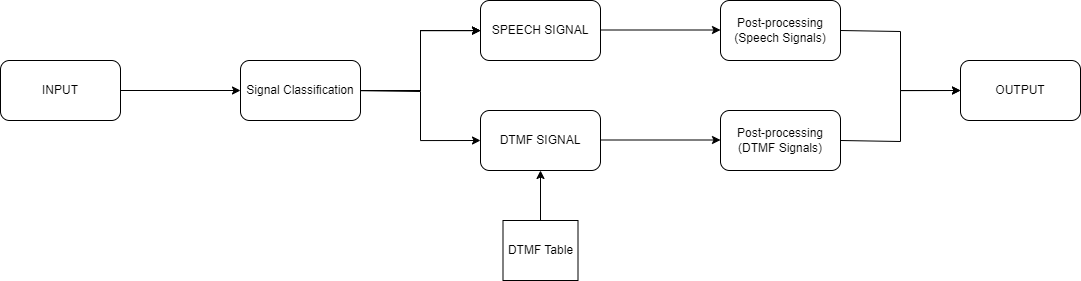
\includegraphics[width=1\linewidth]{FINAL_ASSIGNMENT/A_S_6.png}
    
    
\end{figure}
\subsection{It must be produced in some way that must be specified in the answer! - It is also allowed to use AI (the DTMF signal of the number "x" and add it on top of a voice recording (in your voice!) saying the number "x" so that the DTMF sound is heard together with the voice recording }
\begin{itemize}
    \item The recording (speech + DTMF sound) must be attached and show it in time, in the spectrum and in the spectrogram the number "x" will be the last digit (the check digit) in your ID number.
\end{itemize}

\paragraph{Answer :} 
Since my id is 207370248. the number x is 8 and so i recorded myself saying "Eight".Then, I created a python code that create analog since wave for number 8 which means two frequencies of 852, 1336 hz each. Then, Merged them together and applied spectrogram from $scipy.signal$ library, Results :\\

\begin{figure}[htbp]
    \centering
    \caption{DTMF Signal - Time Domain}
    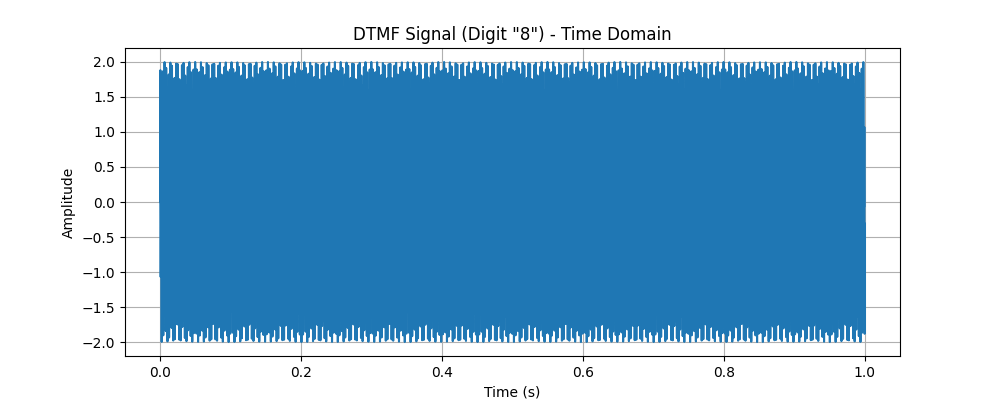
\includegraphics[width=0.75\linewidth]{FINAL_ASSIGNMENT/DTMF Signal - Time Domain.png}
    
    
\end{figure}

\begin{figure}[htbp]
    \centering
        \caption{Voice Recording - Time Domain}

    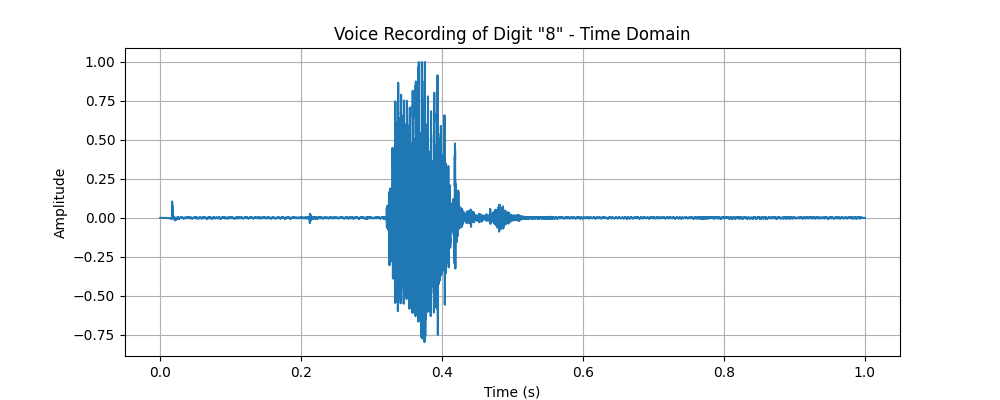
\includegraphics[width=0.75\linewidth]{FINAL_ASSIGNMENT/Voice Recording - Time Domain.png}
    
\end{figure}


\begin{figure}
    \centering
     \caption{Combined Signal - Time Domain}
    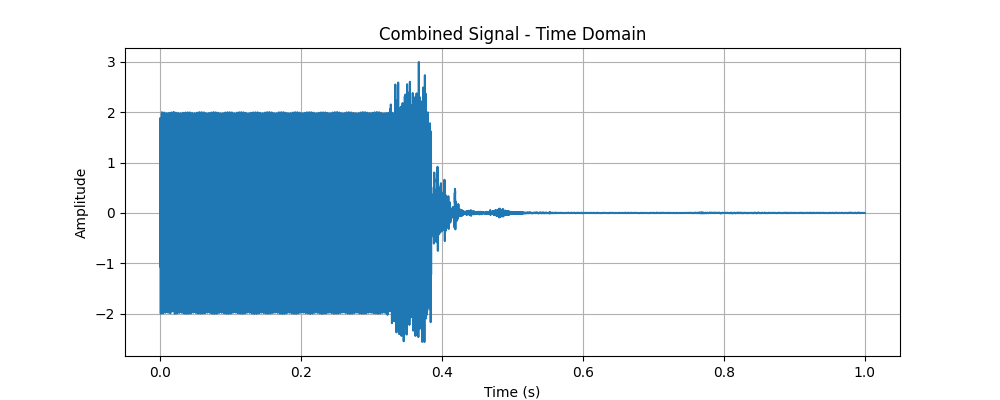
\includegraphics[width=0.75\linewidth]{FINAL_ASSIGNMENT/Combined Signal - Time Domain.png}
   
    
\end{figure}

\begin{figure}
    \centering
        \caption{Spectrogram of Combined Signal}
    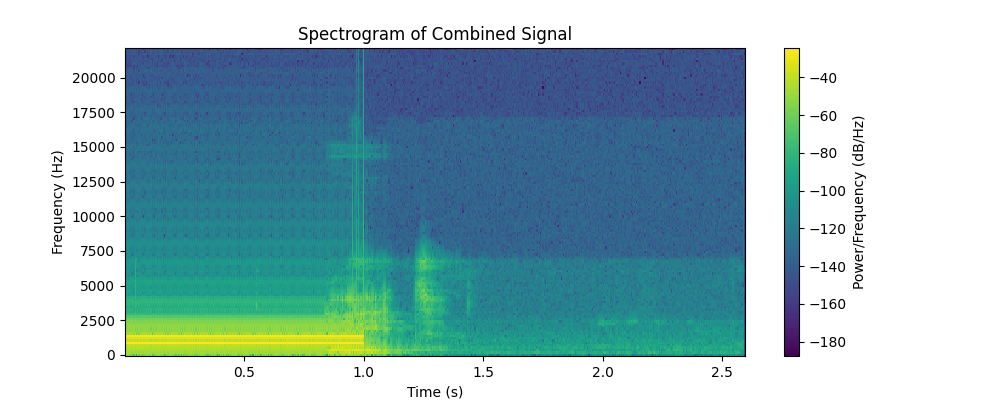
\includegraphics[width=0.75\linewidth]{FINAL_ASSIGNMENT/Spectrogram of Combined Signal.png}
    
\end{figure}

\newpage
\begin{lstlisting}
import numpy as np
import matplotlib.pyplot as plt
from scipy.signal import chirp, spectrogram
import librosa
import librosa.display
from scipy.io import wavfile

output_path = "output/output_"

last_digit_audio_path = "Assignment_3/Recording.wav"
dtmf_audio_path = output_path + "dtmf_audio" + ".wav"
combined_audio_path = output_path + "combined_audio" + ".wav"

def readwav(file_path):
    audio_signal, sample_rate = librosa.load(file_path, sr=None, mono=True)
    bits_per_sample = audio_signal.dtype.itemsize * 8

    return audio_signal, sample_rate, bits_per_sample

def print_info(audio_signal,sample_rate,bits_per_sample):
    print("Audio Signal Shape:", audio_signal.shape)
    print("Sample Rate:", sample_rate)
    print("Bits Per Sample:", bits_per_sample)
    pass

def generate_dtmf_signal(digit, duration, fs):
    dtmf_freqs = {
        '1': (697, 1209), '2': (697, 1336), '3': (697, 1477),
        '4': (770, 1209), '5': (770, 1336), '6': (770, 1477),
        '7': (852, 1209), '8': (852, 1336), '9': (852, 1477),
        '*': (941, 1209), '0': (941, 1336), '#': (941, 1477)
    }
    f1, f2 = dtmf_freqs[digit]
    t = np.linspace(0, duration, int(duration * fs), endpoint=False)
    signal = np.sin(2 * np.pi * f1 * t) + np.sin(2 * np.pi * f2 * t)
    return signal





def Assignment3_Audio():
    print(last_digit_audio_path)
    audio_signal, sample_rate, bits_per_sample = readwav(last_digit_audio_path)
    print_info(audio_signal, sample_rate, bits_per_sample)


    # Parameters
    duration = 1.0  
    fs = 44100  

    dtmf_signal = generate_dtmf_signal('8', duration, fs)

    plt.figure(figsize=(10, 4))
    plt.plot(np.linspace(0, duration, len(dtmf_signal)), dtmf_signal)
    plt.title('DTMF Signal (Digit "8") - Time Domain')
    plt.xlabel('Time (s)')
    plt.ylabel('Amplitude')
    plt.grid(True)
    plt.show()

    wavfile.write(dtmf_audio_path, sample_rate, dtmf_signal)


    voice_recording = audio_signal  

    plt.figure(figsize=(10, 4))
    plt.plot(np.linspace(0, duration, len(voice_recording)), voice_recording)
    plt.title('Voice Recording of Digit "8" - Time Domain')
    plt.xlabel('Time (s)')
    plt.ylabel('Amplitude')
    plt.grid(True)
    plt.show()

    if len(dtmf_signal) < len(voice_recording):
        dtmf_signal = np.pad(dtmf_signal, (0, len(voice_recording) - len(dtmf_signal)), 'constant')
    elif len(dtmf_signal) > len(voice_recording):
        dtmf_signal = dtmf_signal[:len(voice_recording)]

    combined_signal = voice_recording + dtmf_signal

    wavfile.write(combined_audio_path, sample_rate, dtmf_signal)


    plt.figure(figsize=(10, 4))
    plt.plot(np.linspace(0, duration, len(combined_signal)), combined_signal)
    plt.title('Combined Signal - Time Domain')
    plt.xlabel('Time (s)')
    plt.ylabel('Amplitude')
    plt.grid(True)
    plt.show()

    frequencies, spectrum = plt.psd(combined_signal, Fs=fs)

    plt.figure(figsize=(10, 4))
    plt.plot(frequencies, 10 * np.log10(spectrum))
    plt.title('Spectrum of Combined Signal')
    plt.xlabel('Frequency (Hz)')
    plt.ylabel('Power/Frequency (dB/Hz)')
    plt.grid(True)
    plt.show()

    f, t, Sxx = spectrogram(combined_signal, fs)

    plt.figure(figsize=(10, 4))
    plt.pcolormesh(t, f, 10 * np.log10(Sxx))
    plt.title('Spectrogram of Combined Signal')
    plt.xlabel('Time (s)')
    plt.ylabel('Frequency (Hz)')
    plt.colorbar(label='Power/Frequency (dB/Hz)')
    plt.show()

    pass

\end{lstlisting}


\end{document}